\documentclass[journal,12pt,twocolumn]{IEEEtran}
%
\usepackage{setspace}
\usepackage{gensymb}
\usepackage{xcolor}
\usepackage{caption}
%\usepackage{subcaption}
%\doublespacing
\singlespacing

%\usepackage{graphicx}
%\usepackage{amssymb}
%\usepackage{relsize}
\usepackage[cmex10]{amsmath}
\usepackage{mathtools}
%\usepackage{amsthm}
%\interdisplaylinepenalty=2500
%\savesymbol{iint}
%\usepackage{txfonts}
%\restoresymbol{TXF}{iint}
%\usepackage{wasysym}
\usepackage{hyperref}
\usepackage{amsthm}
\usepackage{mathrsfs}
\usepackage{txfonts}
\usepackage{stfloats}
\usepackage{cite}
\usepackage{cases}
\usepackage{subfig}
%\usepackage{xtab}
\usepackage{longtable}
\usepackage{multirow}
%\usepackage{algorithm}
%\usepackage{algpseudocode}
%\usepackage{enumerate}
\usepackage{enumitem}
\usepackage{mathtools}
%\usepackage{iithtlc}
%\usepackage[framemethod=tikz]{mdframed}
\usepackage{listings}


%\usepackage{stmaryrd}


%\usepackage{wasysym}
%\newcounter{MYtempeqncnt}
\DeclareMathOperator*{\Res}{Res}
%\renewcommand{\baselinestretch}{2}
\renewcommand\thesection{\arabic{section}}
\renewcommand\thesubsection{\thesection.\arabic{subsection}}
\renewcommand\thesubsubsection{\thesubsection.\arabic{subsubsection}}

\renewcommand\thesectiondis{\arabic{section}}
\renewcommand\thesubsectiondis{\thesectiondis.\arabic{subsection}}
\renewcommand\thesubsubsectiondis{\thesubsectiondis.\arabic{subsubsection}}

%\renewcommand{\labelenumi}{\textbf{\theenumi}}
%\renewcommand{\theenumi}{P.\arabic{enumi}}

% correct bad hyphenation here
\hyphenation{op-tical net-works semi-conduc-tor}

\lstset{
	language=Python,
	frame=single, 
	breaklines=true,
	columns=fullflexible
}



\begin{document}
	%
	
	\theoremstyle{definition}
	\newtheorem{theorem}{Theorem}[section]
	\newtheorem{problem}{Problem}
	\newtheorem{proposition}{Proposition}[section]
	\newtheorem{lemma}{Lemma}[section]
	\newtheorem{corollary}[theorem]{Corollary}
	\newtheorem{example}{Example}[section]
	\newtheorem{definition}{Definition}[section]
	%\newtheorem{algorithm}{Algorithm}[section]
	%\newtheorem{cor}{Corollary}
	\newcommand{\BEQA}{\begin{eqnarray}}
		\newcommand{\EEQA}{\end{eqnarray}}
	\newcommand{\define}{\stackrel{\triangle}{=}}
	
	\bibliographystyle{IEEEtran}
	%\bibliographystyle{ieeetr}
	
	\providecommand{\nCr}[2]{\,^{#1}C_{#2}} % nCr
	\providecommand{\nPr}[2]{\,^{#1}P_{#2}} % nPr
	\providecommand{\mbf}{\mathbf}
	\providecommand{\pr}[1]{\ensuremath{\Pr\left(#1\right)}}
	\providecommand{\qfunc}[1]{\ensuremath{Q\left(#1\right)}}
	\providecommand{\sbrak}[1]{\ensuremath{{}\left[#1\right]}}
	\providecommand{\lsbrak}[1]{\ensuremath{{}\left[#1\right.}}
	\providecommand{\rsbrak}[1]{\ensuremath{{}\left.#1\right]}}
	\providecommand{\brak}[1]{\ensuremath{\left(#1\right)}}
	\providecommand{\lbrak}[1]{\ensuremath{\left(#1\right.}}
	\providecommand{\rbrak}[1]{\ensuremath{\left.#1\right)}}
	\providecommand{\cbrak}[1]{\ensuremath{\left\{#1\right\}}}
	\providecommand{\lcbrak}[1]{\ensuremath{\left\{#1\right.}}
	\providecommand{\rcbrak}[1]{\ensuremath{\left.#1\right\}}}
	\theoremstyle{remark}
	\newtheorem{rem}{Remark}
	\newcommand{\sgn}{\mathop{\mathrm{sgn}}}
	\providecommand{\abs}[1]{\left\vert#1\right\vert}
	\providecommand{\res}[1]{\Res\displaylimits_{#1}} 
	\providecommand{\norm}[1]{\lVert#1\rVert}
	\providecommand{\mtx}[1]{\mathbf{#1}}
	\providecommand{\mean}[1]{E\left[ #1 \right]}
	\providecommand{\fourier}{\overset{\mathcal{F}}{ \rightleftharpoons}}
	\providecommand{\ztrans}{\overset{\mathcal{Z}}{ \rightleftharpoons}}
	
	%\providecommand{\hilbert}{\overset{\mathcal{H}}{ \rightleftharpoons}}
	\providecommand{\system}{\overset{\mathcal{H}}{ \longleftrightarrow}}
	%\newcommand{\solution}[2]{\textbf{Solution:}{#1}}
	\newcommand{\solution}{\noindent \textbf{Solution: }}
	\providecommand{\dec}[2]{\ensuremath{\overset{#1}{\underset{#2}{\gtrless}}}}
	\numberwithin{equation}{section}
	%\numberwithin{equation}{subsection}
	%\numberwithin{problem}{subsection}
	%\numberwithin{definition}{subsection}
	\makeatletter
	\@addtoreset{figure}{problem}
	\makeatother
	
	\let\StandardTheFigure\thefigure
	%\renewcommand{\thefigure}{\theproblem.\arabic{figure}}
	\renewcommand{\thefigure}{\theproblem}
	
	
	%\numberwithin{figure}{subsection}
	
	\def\putbox#1#2#3{\makebox[0in][l]{\makebox[#1][l]{}\raisebox{\baselineskip}[0in][0in]{\raisebox{#2}[0in][0in]{#3}}}}
	\def\rightbox#1{\makebox[0in][r]{#1}}
	\def\centbox#1{\makebox[0in]{#1}}
	\def\topbox#1{\raisebox{-\baselineskip}[0in][0in]{#1}}
	\def\midbox#1{\raisebox{-0.5\baselineskip}[0in][0in]{#1}}
	
	\vspace{3cm}
	
	\title{ EE 3900 - Assignment 1}
	
	\author{VIBHAVASU}
	
	% make the title area
	\maketitle
	
	%\newpage
	
	\tableofcontents
	
	%\renewcommand{\thefigure}{\thesection.\theenumi}
	%\renewcommand{\thetable}{\thesection.\theenumi}
	
	\renewcommand{\thefigure}{\theenumi}
	\renewcommand{\thetable}{\theenumi}
	
	%\renewcommand{\theequation}{\thesection}
	
	
	\bigskip
	
	\begin{abstract}
		This manual provides a simple introduction to digital signal processing.
	\end{abstract}
	\section{Software Installation}
	Run the following commands
	\begin{lstlisting}
sudo apt-get update
sudo apt-get install libffi-dev libsndfile1 python3-scipy  python3-numpy python3-matplotlib 
sudo pip install cffi pysoundfile 
	\end{lstlisting}
	\section{Digital Filter}
	\begin{enumerate}[label=\thesection.\arabic*
		,ref=\thesection.\theenumi]
		\item
		\label{prob:input}
		Download the sound file from  
		\begin{lstlisting}
wget https://raw.githubusercontent.com/gadepall/EE1310/master/filter/codes/Sound_Noise.wav
		\end{lstlisting}
		%\href{http://tlc.iith.ac.in/img/sound/Sound_Noise.wav}{\url{http://tlc.iith.ac.in/img/sound/Sound_Noise.wav}}  
		%in the link given below.
		%\linebreak
		\item
		\label{prob:spectrogram}
		You will find a spectrogram at \href{https://academo.org/demos/spectrum-analyzer}{\url{https://academo.org/demos/spectrum-analyzer} }. 
		%\end{problem}
		%%
		%
		%%\onecolumn
		%%\input{./figs/fir}
		%\begin{problem}
		Upload the sound file that you downloaded in Problem \ref{prob:input} in the spectrogram  and play.  Observe the spectrogram. What do you find?
		\\
		%
		\solution There are a lot of yellow lines between 440 Hz to 5.1 KHz.  These represent the synthesizer key tones. Also, the key strokes
		are audible along with background noise.
		% By observing spectrogram, it clearly shows that tonal frequency is under 4kHz. And above 4kHz only noise is present.
		\item
		\label{prob:output}
		Write the python code for removal of out of band noise and execute the code.
		\\
		\solution
		\lstinputlisting{./codes/Cancel_noise.py}
		%\begin{figure}[h]
		%\centering
		%\includegraphics[width=\columnwidth]{enc_block_diag.png}
		%\caption{}
		%\label{fig:convolution encoder}
		%\end{figure}
		%\input{block_enc}
		\item
		The output of the python script in Problem \ref{prob:output} is the audio file Sound\_With\_ReducedNoise.wav. Play the file in the spectrogram in Problem \ref{prob:spectrogram}. What do you observe?
		\\
		\solution The key strokes as well as background noise is subdued in the audio.  Also,  the signal is blank for frequencies above 5.1 kHz.
		
	\end{enumerate}
	\section{Difference Equation}
	\begin{enumerate}[label=\thesection.\arabic*,ref=\thesection.\theenumi]
		\item Let
		\begin{equation}
			\label{def:xn}
			x(n) = \cbrak{\underset{\uparrow}{1},2,3,4,2,1}
		\end{equation}
		Sketch $x(n)$.
		\item Let
		\begin{multline}
			\label{eq:iir_filter}
			y(n) + \frac{1}{2}y(n-1) = x(n) + x(n-2), 
			\\
			y(n) = 0, n < 0
		\end{multline}
		Sketch $y(n)$.
		\\
		\solution The following code yields Fig. \ref{fig:xnyn}.
		\begin{lstlisting}
wget https://github.com/gadepall/EE1310/raw/master/filter/codes/xnyn.py
		\end{lstlisting}
		\begin{figure}[!ht]
			\begin{center}
				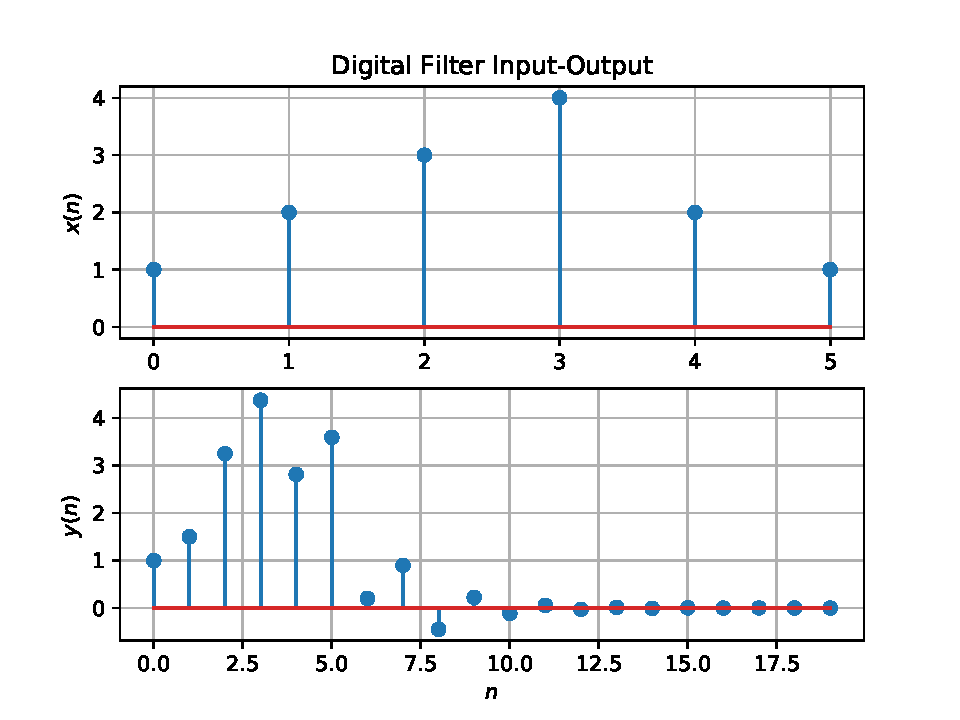
\includegraphics[width=\columnwidth]{./figs/xnyn}
			\end{center}
			\captionof{figure}{}
			\label{fig:xnyn}	
		\end{figure}
		
		\item Repeat the above exercise using a C code.
		\solution: C Code
		\begin{lstlisting}
wget https://github.com/DarkWake9/EE3900/blob/main/Assignment%201/e3-3.c
		\end{lstlisting}
		\solution: Python Code
\begin{lstlisting}
wget https://github.com/DarkWake9/EE3900/blob/main/Assignment%201/e3-3.py
\end{lstlisting}		
	\end{enumerate}
	\section{$Z$-transform}
	\begin{enumerate}[label=\thesection.\arabic*]
		\item The $Z$-transform of $x(n)$ is defined as
		%
		\begin{equation}
			\label{eq:z_trans}
			X(z)={\mathcal {Z}}\{x(n)\}=\sum _{n=-\infty }^{\infty }x(n)z^{-n}
		\end{equation}
		%
		Show that
		\begin{equation}
			\label{eq:shift1}
			{\mathcal {Z}}\{x(n-1)\} = z^{-1}X(z)
		\end{equation}
		and find
		\begin{equation}
			{\mathcal {Z}}\{x(n-k)\} 
		\end{equation}
		\solution From \eqref{eq:z_trans},
		\begin{align}
			{\mathcal {Z}}\{x(n-k)\} &=\sum _{n=-\infty }^{\infty }x(n-1)z^{-n}
			\\
			&=\sum _{n=-\infty }^{\infty }x(n)z^{-n-1} = z^{-1}\sum _{n=-\infty }^{\infty }x(n)z^{-n}
		\end{align}
		resulting in \eqref{eq:shift1}. Similarly, it can be shown that
		%
		\begin{equation}
			\label{eq:z_trans_shift}
			{\mathcal {Z}}\{x(n-k)\} = z^{-k}X(z)
		\end{equation}
		\item Obtain $X(z)$ for $x(n)$ defined in problem 
		\ref{def:xn}.
		\item Find
		%
		\begin{equation}
			H(z) = \frac{Y(z)}{X(z)}
		\end{equation}
		%
		from  \eqref{eq:iir_filter} assuming that the $Z$-transform is a linear operation.
		\\
		\solution  Applying \eqref{eq:z_trans_shift} in \eqref{eq:iir_filter},
		\begin{align}
			Y(z) + \frac{1}{2}z^{-1}Y(z) &= X(z)+z^{-2}X(z)
			\\
			\implies \frac{Y(z)}{X(z)} &= \frac{1 + z^{-2}}{1 + \frac{1}{2}z^{-1}}
			\label{eq:freq_resp}
		\end{align}
		%
		\item Find the Z transform of 
		\begin{equation}
			\delta(n)
			=
			\begin{cases}
				1 & n = 0
				\\
				0 & \text{otherwise}
			\end{cases}
		\end{equation}
		and show that the $Z$-transform of
		\begin{equation}
			\label{eq:unit_step}
			u(n)
			=
			\begin{cases}
				1 & n \ge 0
				\\
				0 & \text{otherwise}
			\end{cases}
		\end{equation}
		is
		\begin{equation}
			U(z) = \frac{1}{1-z^{-1}}, \quad \abs{z} > 1
		\end{equation}
		\solution It is easy to show that
		\begin{equation}
			\delta(n) \ztrans 1
		\end{equation}
		and from \eqref{eq:unit_step},
		\begin{align}
			U(z) &= \sum _{n= 0}^{\infty}z^{-n}
			\\
			&=\frac{1}{1-z^{-1}}, \quad \abs{z} > 1
		\end{align}
		using the fomula for the sum of an infinite geometric progression.
		%
		\begin{enumerate}[label=(\roman*)]
			\item \solution \begin{equation}
				\Delta(z) = z\{\delta[n]\}=\sum_{n=-\infty}^{\infty} \delta(n) z^{-n} = 1\\
			\end{equation}
			
			\item \solution \begin{align}
				U(z) = Z\{\delta(n)\}=\sum_{n=-\infty}^{\infty} u[n] z^{-n} \\
				=1+z^{-1}+z^{-2}+\cdots \\
				=\frac{1}{1-z^{-1}}
			\end{align}
		\end{enumerate}
		
		\item Show that 
		\begin{equation}
			\label{eq:anun}
			a^nu(n) \ztrans \frac{1}{1-az^{-1}} \quad \abs{z} > \abs{a}
		\end{equation}
		
		\solution
		\begin{align}
			a^{n}u[n] = \begin{cases} a^{n} & n \geq 0 \\
				0 & n<0\end{cases} \\
			U^{\prime}(z)={\mathcal{Z}}\{a^{n}u[n]\}=\sum_{n=-\infty}^{\infty} a^{n}[n] z^{-n}
		\end{align}
		\begin{equation}
			\label{eq:U'}
			U^{\prime}(z)=\frac{1}{1-a z^{-1}}
		\end{equation}
		
		
		\item 
		Let
		\begin{equation}
			H\brak{e^{\j \omega}} = H\brak{z = e^{\j \omega}}.
		\end{equation}
		Plot $\abs{H\brak{e^{\j \omega}}}$.  Is it periodic? If so, find the period. $H(e^{\j \omega})$ is
		known as the {\em Discret Time Fourier Transform} (DTFT) of $x(n)$.
		\\[10pt]
		\solution The following code plots Fig. \ref{fig:dtft}.
		\begin{lstlisting}
wget https://raw.githubusercontent.com/gadepall/EE1310/master/filter/codes/dtft.py
		\end{lstlisting}
		\begin{figure}[!ht]
			\centering
			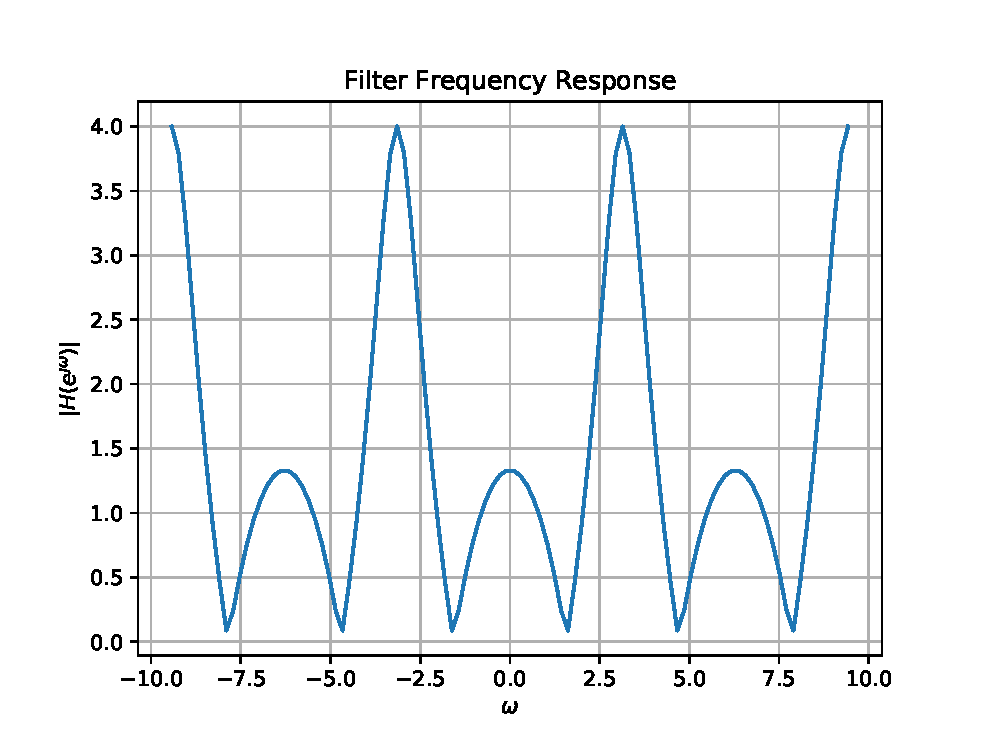
\includegraphics[width=\columnwidth]{./figs/dtft}
			\caption{$\abs{H\brak{e^{\j\omega}}}$}
			\label{fig:dtft}
		\end{figure}\\[200pt]
	
	\item Express $h(n)$ in terms of $H\brak{e^{\j \omega}}$.\\
	\solution
		\begin{align}
	H( e^{j\omega }) =\sum ^{\infty }_{n=-\infty }h(n') e^{-j\omega n'}\\
	\implies \int_{\-\pi} ^{\pi }	H\left( e^{j\omega }\right) e^{j\omega n}d\omega\\			
	= \sum_{n'=-\infty }^{\infty } \int ^{\pi }_{-\pi }h(n') e^{-j\omega n'}e^{j\omega n}d\omega\\			
	=\sum ^{\infty }_{n'=-\infty }h(n') 2\pi \delta(n'- n) =
	 2\pi h(n) 
		\end{align}
	\begin{equation}
		\therefore	 h(n) =\dfrac{1}{2\pi }\int ^{\pi }_{-\pi }H\left( e^{ja}\right) e^{j\omega }d\omega 
	\end{equation}

	\end{enumerate}
	
	\section{Impulse Response}
	\begin{enumerate}[label=\thesection.\arabic*]
		\item \label{prob:impulse_resp}
		Find an expression for $h(n)$ using $H(z)$, given that 
		%in Problem \ref{eq:ztransab} and \eqref{eq:anun}, given that
		\begin{equation}
			\label{eq:impulse_resp}
			h(n) \ztrans H(z)
		\end{equation}
		and there is a one to one relationship between $h(n)$ and $H(z)$. $h(n)$ is known as the {\em impulse response} of the
		system defined by \eqref{eq:iir_filter}.
		\\
		\solution From \eqref{eq:freq_resp},
		\begin{align}
			H(z) &= \frac{1}{1 + \frac{1}{2}z^{-1}} + \frac{ z^{-2}}{1 + \frac{1}{2}z^{-1}}
			\\
			\implies h(n) &= \brak{-\frac{1}{2}}^{n}u(n) + \brak{-\frac{1}{2}}^{n-2}u(n-2)
		\end{align}
		using \eqref{eq:anun} and \eqref{eq:z_trans_shift}.
		\item Sketch $h(n)$. Is it bounded? Convergent? 
		\\
		\solution The following code plots Fig. \ref{fig:hn}.
		\begin{lstlisting}
wget https://raw.githubusercontent.com/gadepall/EE1310/master/filter/codes/hn.py
		\end{lstlisting}
		\begin{figure}[!ht]
			\centering
			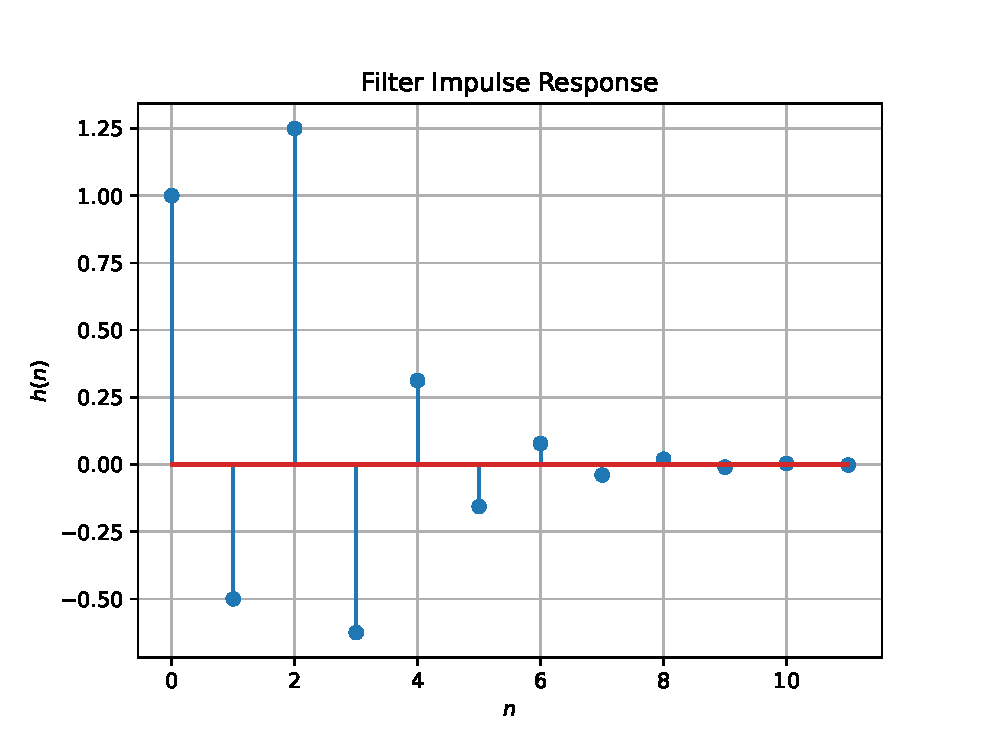
\includegraphics[width=\columnwidth]{./figs/hn}
			\caption{$h(n)$ as the inverse of $H(z)$}
			\label{fig:hn}
		\end{figure}
		\item The system with $h(n)$ is defined to be stable if
		\begin{equation}
			\sum_{n=-\infty}^{\infty}h(n) < \infty
		\end{equation}
		Is the system defined by \eqref{eq:iir_filter} stable for the impulse response in \eqref{eq:impulse_resp}?
		%
		\item 
		Compute and sketch $h(n)$ using 
		\begin{equation}
			\label{eq:iir_filter_h}
			h(n) + \frac{1}{2}h(n-1) = \delta(n) + \delta(n-2), 
		\end{equation}
		%
		This is the definition of $h(n)$.
		\\
		\solution The following code plots Fig. \ref{fig:hndef}. Note that this is the same as Fig. 
		\ref{fig:hn}. 
		\begin{lstlisting}
wget https://raw.githubusercontent.com/gadepall/EE1310/master/filter/codes/hndef.py
		\end{lstlisting}
		\begin{figure}[!ht]
			\centering
			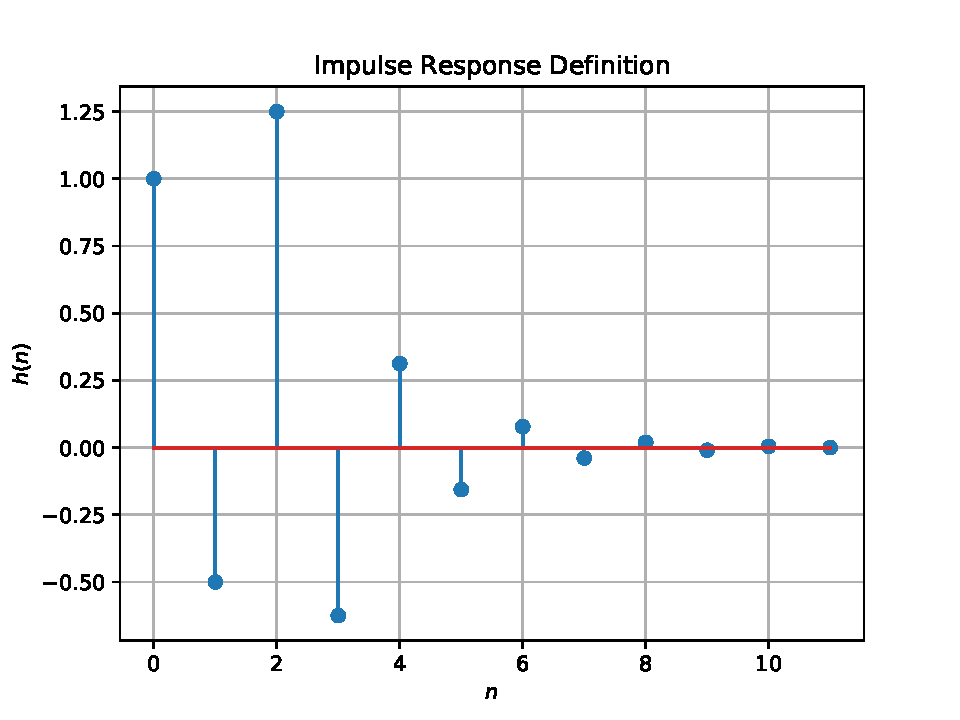
\includegraphics[width=\columnwidth]{./figs/hndef}
			\caption{$h(n)$ from the definition}
			\label{fig:hndef}
		\end{figure}
		\\[100pt]
		\item Compute 
		%
		\begin{equation}
			\label{eq:convolution}
			y(n) = x(n)*h(n) = \sum_{n=-\infty}^{\infty}x(k)h(n-k)
		\end{equation}
		
		Comment. The operation in \eqref{eq:convolution} is known as
		{\em convolution}.
		
		\solution The following code plots Fig. \ref{fig:ynconv}. Note that this is the same as 
		$y(n)$ in  Fig. 
		\ref{fig:xnyn}. 
		%
		\begin{lstlisting}
wget https://raw.githubusercontent.com/gadepall/EE1310/master/filter/codes/ynconv.py
		\end{lstlisting}
		\begin{figure}[!ht]
			\centering
			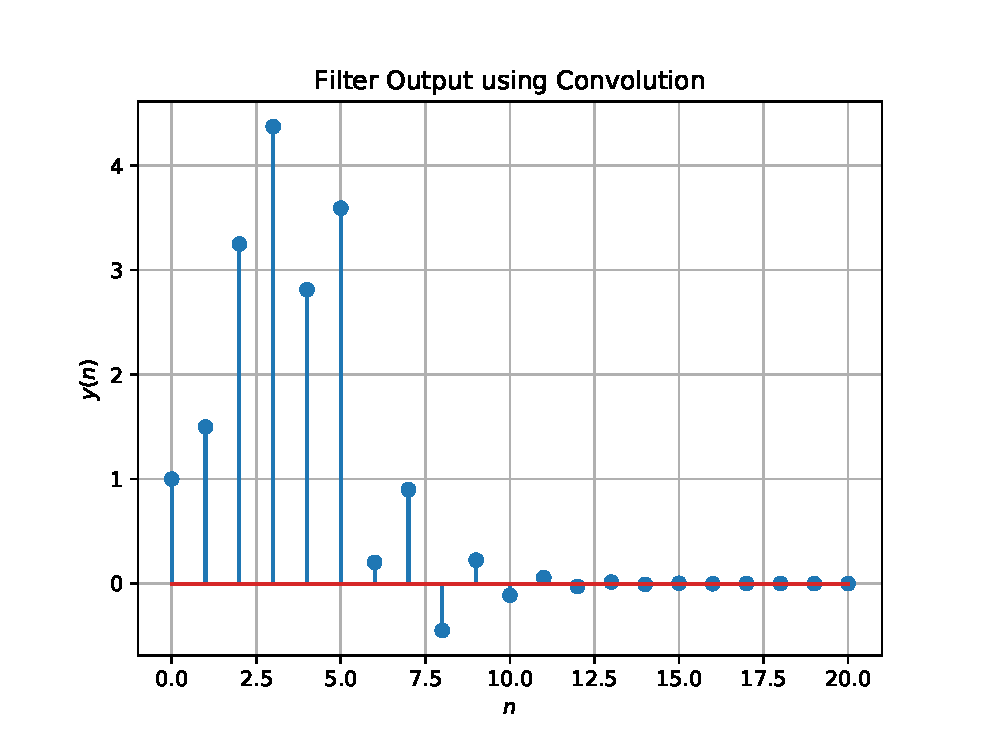
\includegraphics[width=\columnwidth]{./figs/ynconv}
			\caption{$y(n)$ from the definition of convolution}
			\label{fig:ynconv}
		\end{figure}
		
		\item Show that
		\begin{equation}
			y(n) =  \sum_{n=-\infty}^{\infty}x(n-k)h(k)
		\end{equation}
		
		5.6 \solution
		\begin{align}
			%	y(n)=\sum_{n=-\infty}^{\infty} x(n-k) h(k) \\
			%	\text{6.2 To prove: } Y(k)=X(k) H(k)\\
			X(z) = {\mathcal{Z}} \{x(n)\}=\sum_{n=-\infty}^{\infty} x(n) z^{-n} \\
			H(z) = {\mathcal{Z}} \{h(m)\}=\sum_{m=-\infty}^{\infty} h(m) z^{-m}\right.
		\end{align}
		
		\begin{equation}
			X(z) H(z)=\sum_{n=-\infty}^{\infty} x(n) z^{-n} \sum_{m=-\infty}^{\infty} h(m) z^{-m}
		\end{equation}
		
		\begin{align}
			=\sum_{n=-\infty}^{\infty} \sum_{m=-\infty}^{\infty} x[n] h[m] z^{-(n+m)} \\
			\intertext{Let $m = k - n$}	%\quad m=-\infty \rightarrow n=\infty \\
			%m=\infty \rightarrow n=-\infty \\
			=\sum_{k=-\infty}^{\infty}\left(\sum_{n=-\infty}^{\infty} x[n] h[n-k]\right) z^{-k} \\
			=\sum_{k=-\infty}^{\infty} y[n] z^{-k}=Y({$z$}) \\
			\implies Y(z)= X(z) \cdot H(z)\\
			%	Y(z)=\sum_{n=-\infty}^{\infty} x(n) \sum_{m=-\infty}^{\infty} h(m) z^{-(m+n)} \\
			%	\text{Let } m = n - k \\
			%	\implies Y(z)=\sum_{n=-\infty}^{\infty} \left( \sum_{n=-\infty}^{\infty} x(n) h(n-k) z^{-k} \right). \\
		\end{align}
		
		now put $n+m=k \quad n=-\infty$
		
		\begin{align}
			\Rightarrow Y(z)=\sum_{k=-\infty}^{\infty} x(m-k) \sum_{m=-\infty}^{\infty} h(m) z^{-k} \\
			=\sum_{k=-\infty}^{\infty}\left(\sum_{m=-\infty}^{\infty} x[m-k] h[k]\right) z^{-k} \\
			\text { but } Y(z)=\sum_{k=-\infty}^{\infty} y(m) z^{-k} \\
			\Rightarrow y(m)=\sum_{m=-\infty}^{\infty} x[m-k] h(k) \\
			5 \cdot 6 \rightarrow y(n)=\sum_{n=-\infty}^{\infty} x(n-k) h(k) 
		\end{align}
		
	\end{enumerate}
	
	%
	\section{DFT and FFT}
	\begin{enumerate}[label=\thesection.\arabic*]
		\item
		Compute
		\begin{equation}
			X(k) \define \sum _{n=0}^{N-1}x(n) e^{-\j2\pi kn/N}, \quad k = 0,1,\dots, N-1
		\end{equation}
		and $H(k)$ using $h(n)$.
		\item Compute 
		\begin{equation}
			Y(k) = X(k)H(k)
		\end{equation}
		\item Compute
		\begin{equation}
			y\brak{n}={\frac {1}{N}}\sum _{k=0}^{N-1}Y\brak{k}\cdot e^{\j 2\pi kn/N},\quad n = 0,1,\dots, N-1
		\end{equation}
		\\
		\solution The following code plots Fig. \ref{fig:ynconv}. Note that this is the same as 
		$y(n)$ in  Fig. 
		\ref{fig:xnyn}. 
		\\[5pt]
		\begin{lstlisting}
wget https://raw.githubusercontent.com/gadepall/EE1310/master/filter/codes/yndft.py
		\end{lstlisting}
		\begin{figure}[!ht]
			\centering
			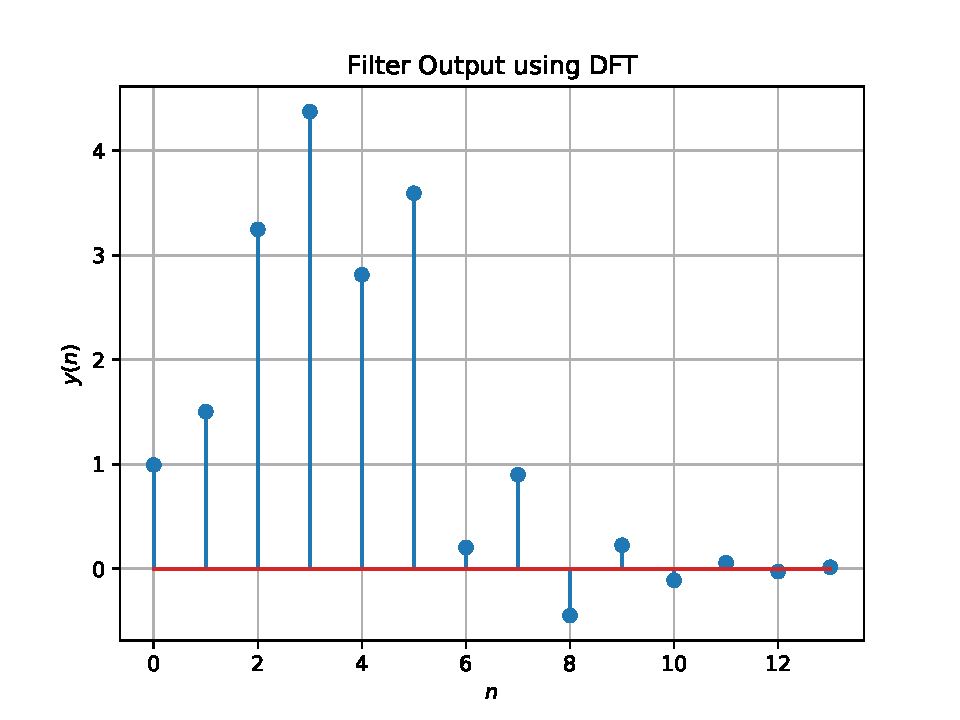
\includegraphics[width=\columnwidth]{./figs/yndft}
			\caption{$y(n)$ from the DFT}
			\label{fig:yndft}
		\end{figure}
		
		\item Repeat the previous exercise by computing $X(k), H(k)$ and $y(n)$ through FFT and 
		IFFT.
		\item Wherever possible, express all the above equations as matrix equations.
	\end{enumerate}
	%
	\section{Exercises}
	
	Answer the following questions by looking at the python code in Problem \ref{prob:output}.
	\begin{enumerate}[label=\thesection.\arabic*]
		\item
		The command
		\begin{lstlisting}
output_signal = signal.lfilter(b, a, input_signal)
		\end{lstlisting}
		in Problem \ref{prob:output} is executed through the following difference equation
		\begin{equation}
			\label{eq:iir_filter_gen}
			\sum _{m=0}^{M}a\brak{m}y\brak{n-m}=\sum _{k=0}^{N}b\brak{k}x\brak{n-k}
		\end{equation}
		%
		where the input signal is $x(n)$ and the output signal is $y(n)$ with initial values all 0. Replace
		\textbf{signal.filtfilt} with your own routine and verify.
		%
		\item Repeat all the exercises in the previous sections for the above $a$ and $b$.
		
		\item What is the sampling frequency of the input signal?
		\\
		\solution
		Sampling frequency(fs)=44.1kHZ.
		\item
		What is type, order and  cutoff-frequency of the above butterworth filter
		\\
		\solution
		The given butterworth filter is low pass with order=2 and cutoff-frequency=4kHz.
		%
		\item
		Modifying the code with different input parameters and to get the best possible output.
		%
	\end{enumerate}
	
\end{document}

